\documentclass[11pt]{article}

\usepackage[utf8]{inputenc}
\usepackage[T1]{fontenc}
\usepackage{lmodern}
\usepackage[margin=1in]{geometry}
\usepackage{graphicx}
\graphicspath{{figures/}}
\usepackage{booktabs}
\usepackage{amsmath}
\usepackage{amssymb}
\usepackage{microtype}
\usepackage{xcolor}
\usepackage[numbers,sort&compress]{natbib}
\usepackage[hidelinks]{hyperref}
\usepackage{caption}

\title{\textbf{Detection Is Not Action:}\\
The Detectability Boundary of Pre-training Data-Readiness Gating}
\author{Gargi Desai\\\texttt{gargi.desai20@gmail.com}}
\date{}

\begin{document}
\maketitle

\begin{abstract}
Many high-stakes AI failures trace to the training data rather than the model, yet
teams still treat pre-training data validation as a checklist and rarely wire its
signals to a go/no-go decision or to a governance framework. We study the
\emph{detectability boundary} of that validation: what a pre-training
data-readiness gate catches, what it misses, and why a \emph{flagged} source is
often not \emph{blocked}. We reuse a validation gate from a prior single-domain
system and generalize it across three high-stakes domains (healthcare, finance,
and government) on the real MIMIC-IV, SEC EDGAR, and CMS Open Payments datasets,
injecting controlled defects across simulated sources. A composite readiness score
detects $0.76$ of degraded sources (95\% CI $[0.74,0.76]$) but withholds only
$0.42$; the $0.34$ gap (95\% CI $[0.32,0.35]$) traces to a single averaging step,
and we show it is fixable but privacy-sensitive. The grid is small by design (six
sources per domain, two degraded, five seeds), so the intervals describe this
controlled setting, not field variability. We map the privacy--utility curve of
validating on differentially private summaries, prove a blind spot for symmetric
label noise on balanced targets, and add a confident-learning label detector that
runs on DP-noised summaries and keeps its recall down to $\varepsilon{=}0.1$. We
compare against Great Expectations and Deequ, measure how poorly thresholds port
across domains, and map the gate to the NIST AI RMF MEASURE function. We report the
negatives, among them a near-chance inter-rater reliability on fine-grained
incident coding. What is new is the integration of production incidents, a private
benchmarked gate, and a governance mapping, not any one of those parts.
\end{abstract}

\section{Introduction}

A large share of real-world AI failures come from the data rather than the model,
and the point that data quality matters is by now well
established~\citep{sambasivan2021datacascades,sculley2015debt}. The AI Incident
Database~\citep{mcgregor2021aiid} catalogues such failures, and taxonomies of them
exist~\citep{paeth2024aiid}. This paper adds neither another incident taxonomy nor
another argument that data quality matters. It is an \textbf{integration}: we
connect (i) production incidents, used only to ground which failure modes are worth
testing, (ii) a private, cross-source, pre-training \emph{validation gate}
benchmarked across three high-stakes domains, and (iii) the NIST AI Risk Management
Framework's MEASURE function~\citep{nistairmf2023}, the governance regime that
high-stakes deployments answer to~\citep{euaiact2024,isoiec42001}.

This is a \emph{detectability-boundary study}, not a ``we built a gate and it
works'' tool paper, and our own measurements force that framing. The gate gives no
downstream accuracy lift (we find none). It gives a clear account of what
pre-training validation catches, what it misses, and where measuring a problem
parts ways with acting on it. That divergence is the central result: a composite
readiness score detects far more bad data than it withholds. We show why that
happens and what the fix costs.

\paragraph{Contributions.}
\begin{enumerate}
\item \textbf{The spine (detection $\neq$ action).} Across three domains the gate
  detects $0.76$ of degraded sources but withholds only $0.42$ (a $0.34$ gap, 95\%
  CI $[0.32,0.35]$), because a weighted-mean readiness score averages away a severe
  single-dimension defect. We report detection and action as separate metrics
  throughout and, through a decision-rule ablation, show the gap is a \emph{fixable}
  design choice whose fix reintroduces sensitivity to differential-privacy noise.
\item \textbf{A privacy--utility characterization} of validating on differentially
  private summaries, with a usable budget range, and a \emph{confident-learning}
  label detector~\citep{northcutt2021confidentlearning} that runs on DP-noised
  summaries, closes a provable blind spot (symmetric label noise on balanced
  targets), and keeps its recall to $\varepsilon{=}0.1$.
\item \textbf{Honest boundaries and baselines}: a cross-domain threshold transfer
  that fails on precision rather than recall; a comparison with Great Expectations
  and Deequ that places the gate's edge in the integration layer rather than the
  individual checks; and a near-chance inter-rater reliability on fine incident
  coding that we report rather than hide.
\item \textbf{A MEASURE mapping} that ties the measured behaviors to specific NIST
  AI RMF subcategories as governance-facing connective tissue.
\end{enumerate}

\section{Related work}\label{sec:related}

\paragraph{Data readiness and documentation.}
\citet{lawrence2017datareadiness} introduced qualitative Data Readiness Levels
(accessibility / validity / utility) for communicating about data maturity; the
IBM Data Readiness Report~\citep{afzal2020datareadinessreport} generates
dataset-level readiness documentation. We \emph{operationalize} readiness as a
quantitative, benchmarked gate decision and expose a failure mode (composite
masking) that qualitative levels and human-facing reports cannot surface. Dataset
and model documentation standards~\citep{gebru2021datasheets,mitchell2019modelcards,bender2018datastatements}
and the data-centric-AI program~\citep{zha2023datacentric} motivate the frame but
do not benchmark a gating decision.

\paragraph{Data validation systems.}
\citet{breck2019datavalidation} present the canonical ML data-validation line (the
system behind TensorFlow Data Validation), and Deequ~\citep{schelter2018deequ} and
Great Expectations~\citep{greatexpectations} provide declarative ``unit tests for
data'' at scale. These are our baselines, not our contribution: we reuse their
style of check and show (\S\ref{sec:baselines}) that the gate matches them on the
checks they are built for while adding a cross-source, differentially private
\emph{decision} layer. We turn that line's per-source signals into a composite gate
and show the aggregation hides severe single-dimension defects.

\paragraph{Privacy-preserving data quality in federated settings.}
LIA~\citep{rokvic2022lia} evaluates data quality in federated learning by sending
differentially private, lazy-influence scores to a coordinator (recall $>$90\% at
$\varepsilon\leq1$). LIA scores data by its \emph{influence on the model}; our gate
validates against expectation suites (schema / completeness / distribution /
label) and its contribution is the detectability-boundary and masking analysis.
AIDRIN~\citep{hiniduma2025aidrin} is the nearest neighbor: an AI-data-readiness
\emph{reporter} that computes per-dimension metrics (completeness, class imbalance,
fairness, privacy) for a human and, in its 2.0 version, integrates with
privacy-preserving federated learning. AIDRIN \emph{reports}; we \emph{decide}. We
then show that the composite gating \emph{decision} masks single-dimension defects,
which a report-only architecture does not produce. We treat these as positioning
anchors to differentiate from, not components we reuse.

\paragraph{This work vs.\ the closest prior art.}
Against~\citet{sambasivan2021datacascades} (data cascades): they show data
problems propagate; we provide a \emph{measured decision boundary} for catching
them before training. Against the AIID line~\citep{mcgregor2021aiid,paeth2024aiid}:
they classify \emph{causes}; we ask the narrower, operational question of
\emph{pre-training detectability} and connect it to a gate and to MEASURE.

\section{The readiness gate}\label{sec:gate}

The gate is reused unmodified from a prior single-domain system (``FedCheck'',
the validated instantiation; unpublished); this paper generalizes it across
domains and maps it to governance. It never sees raw rows, only noised metadata
reports, which lets it operate in restricted-data settings such as MIMIC-IV under a
data-use agreement.

\paragraph{Per-source checks.} Each source emits a quality report: schema and
dtype checks, per-column null-fraction checks, and (given a label column) a noised
positive-label rate. Reports carry metadata only.

\paragraph{Cross-source consensus.} Distributional drift is detected by comparing
each source's noised feature histograms to the cross-source consensus using the
Jensen--Shannon divergence~\citep{jensenshannon}; a source exceeding a per-domain
\texttt{divergence\_threshold} is flagged. A one-sided label-rate consensus check
flags sources whose positive rate departs from the median.

\paragraph{Differential privacy.} Every released statistic is differentially
private via the Laplace mechanism~\citep{dwork2014}; the privacy budget
$\varepsilon$ is swept in all experiments. DP lets a source contribute validation
signal without exposing rows.

\paragraph{Composite readiness score and decision.} A source's readiness is the
weighted mean
\[
  \text{score} = 0.4\cdot\text{pass\_rate} + 0.3\cdot\text{schema} + 0.3\cdot\text{divergence\_score},
\]
with decision \textsc{ready} ($\geq 0.8$), \textsc{fixable} ($\geq 0.5$), or
\textsc{exclude} (below, or schema-incompatible). This averaging is the mechanism
behind the central finding (\S\ref{sec:spine}): one failed check out of
${\sim}15$ moves \texttt{pass\_rate} only $1.00\!\to\!0.93$, which the $0.4$ weight
absorbs, so a flagged source still scores \textsc{ready}.

\section{Experimental setup}\label{sec:setup}

\paragraph{Domains (real data).} Healthcare: MIMIC-IV in-hospital
mortality~\citep{mimiciv} (DUA-restricted, used read-only, aggregates only).
Finance: SEC EDGAR adverse-earnings from quarterly
filings~\citep{secedgar}. Government: CMS Open Payments food-and-beverage
classification~\citep{cmsopenpayments}.

\paragraph{Degradation taxonomy.} Four pre-training-detectable, row-injectable
modes grounded in production incidents: \emph{structural} (drop/corrupt a column),
\emph{completeness} (null a fraction of a column), \emph{distributional}
(scale-shift a feature), and \emph{label} (flip labels). Each is injected into a
subset of simulated sources at low/med/high severity.

\paragraph{Grid and metrics.} For each domain $\times$ mode $\times$ severity
$\times$ $\varepsilon\in\{0.1,0.5,1,5,\infty\}$ $\times$ seed (0--4), with
$6$ sources of which $2$ are degraded, we record per-mode detection
precision/recall, the gate's \textsc{ready}/\textsc{fixable}/\textsc{exclude}
decisions, the clean-source false-flag rate, and downstream metrics on a clean
holdout. Fixed seeds; every results file records its reproduction command.
\textbf{Detection} (a check fired) and \textbf{action} (the decision withheld the
source) are reported as separate quantities throughout. Confidence intervals are
seed-level percentile bootstraps (10k resamples).

\section{Results}

\subsection{The spine: detection is not action}\label{sec:spine}

The paper's central result is a gap between what the gate \emph{detects} and what
it \emph{acts on}. Aggregated over all three domains at $\varepsilon{=}\infty$
(Fig.~\ref{fig:spine}), the gate detects $0.76$ of degraded sources
(95\% CI $[0.74,0.76]$) but withholds only $0.42$. The $0.34$ difference
(95\% CI $[0.32,0.35]$; seed-level bootstrap, 10k resamples) has a confidence
interval that excludes zero by a wide margin, so it is a property of the decision
rule, not seed noise. Counted per grid cell, $74$ of $180$ degraded cells ($41\%$)
are detected but never withheld.

Table~\ref{tab:spine} shows where the gap opens. For \emph{structural} defects the
gate detects and withholds at $1.00$ in every domain. For \emph{completeness} and
\emph{distributional} defects in finance and government it detects at
$0.73$--$1.00$ yet withholds $0.00$: it sees the defect and still passes the source
as \textsc{ready}. \emph{Label} defects are withheld at $0.00$ in all three domains.
The only modes the gate reliably \emph{acts} on are structural (hard schema
exclusion) and, in healthcare, completeness and distributional defects that happen
to trip other checks. This is the $\varepsilon{=}\infty$ slice, so the cause is the
composite averaging of \S\ref{sec:gate}, not privacy noise.

\begin{figure}[t]
\centering
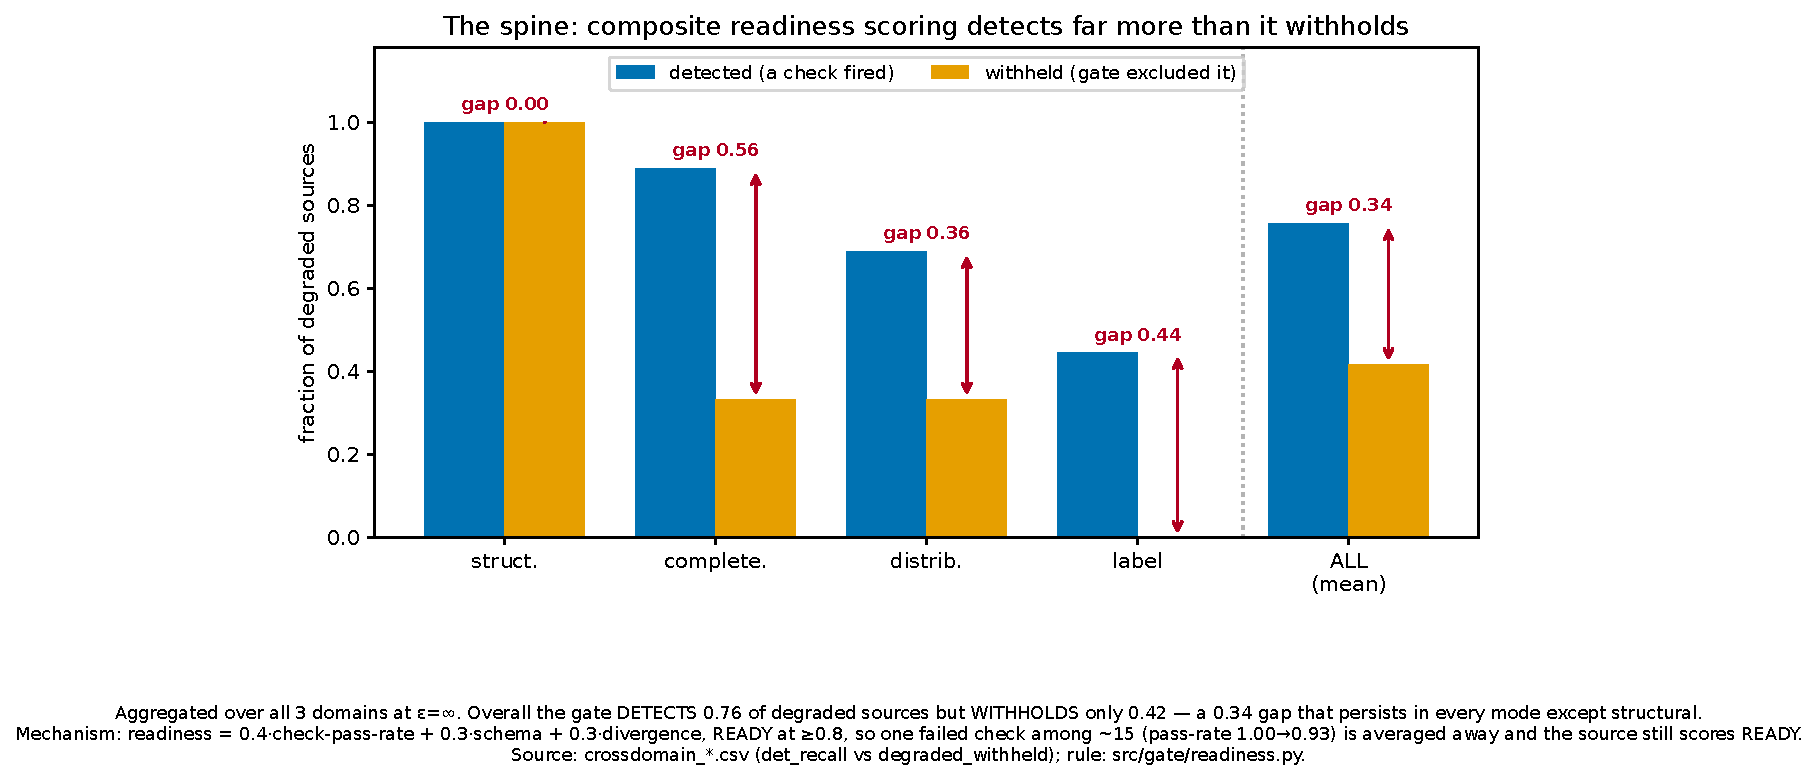
\includegraphics[width=0.82\textwidth]{fig6_detection_action_gap.pdf}
\caption{\textbf{The spine.} Per mode (and overall) the gate detects far more
degraded sources than it withholds; whiskers are seed-level bootstrap 95\% CIs.
The gap is near-zero only for structural defects.}
\label{fig:spine}
\end{figure}

\begin{table}[t]
\centering
\caption{Detection vs.\ gate action at $\varepsilon{=}\infty$, by degradation mode
and domain (means over 5 seeds $\times$ 3 severities per cell, from
\texttt{metrics\_summary.csv}). \emph{det} = detection recall (a check fired);
\emph{act} = fraction of degraded sources the decision actually withheld.
\textbf{det\,$>$\,act is the spine}: the gate saw the defect and still passed the
source. Boldface marks the masked cells (positive detection, zero action).}
\label{tab:spine}
\small
\begin{tabular}{lcccccc}
\toprule
 & \multicolumn{2}{c}{Healthcare} & \multicolumn{2}{c}{Finance} & \multicolumn{2}{c}{Government} \\
\cmidrule(lr){2-3}\cmidrule(lr){4-5}\cmidrule(lr){6-7}
Mode & det & act & det & act & det & act \\
\midrule
Structural     & 1.00 & 1.00 & 1.00 & 1.00 & 1.00 & 1.00 \\
Completeness   & 0.67 & 1.00 & 1.00 & \textbf{0.00} & 1.00 & \textbf{0.00} \\
Distributional & 0.33 & 1.00 & 0.73 & \textbf{0.00} & 1.00 & \textbf{0.00} \\
Label          & 0.67 & \textbf{0.00} & 0.00 & 0.00 & 0.67 & \textbf{0.00} \\
\bottomrule
\end{tabular}
\end{table}

\paragraph{The gap is a fixable but privacy-sensitive design choice.}
Re-deciding the \emph{same} reports under alternative rules (Fig.~\ref{fig:ablation})
shows a \texttt{any-critical} rule (any failed check $\rightarrow$ exclude) drives
the gap to $0.00$ on finance and government (from $0.43$ and $0.67$ respectively),
while a \texttt{max-violation} rule is only a partial fix. However, the clean
false-positive rate of \texttt{any-critical} is $0.000$ for $\varepsilon\geq1$,
$0.011$ at $\varepsilon{=}0.5$, but $0.878$ at $\varepsilon{=}0.1$: the averaging
that \emph{causes} the masking is the same averaging that makes the composite
robust to DP noise. The masking is fixable for $\varepsilon\geq0.5$ at no
false-positive cost; below that, a privacy$\leftrightarrow$aggregation tradeoff
remains. (No threshold was tuned on the outcome.)

\begin{figure}[t]
\centering
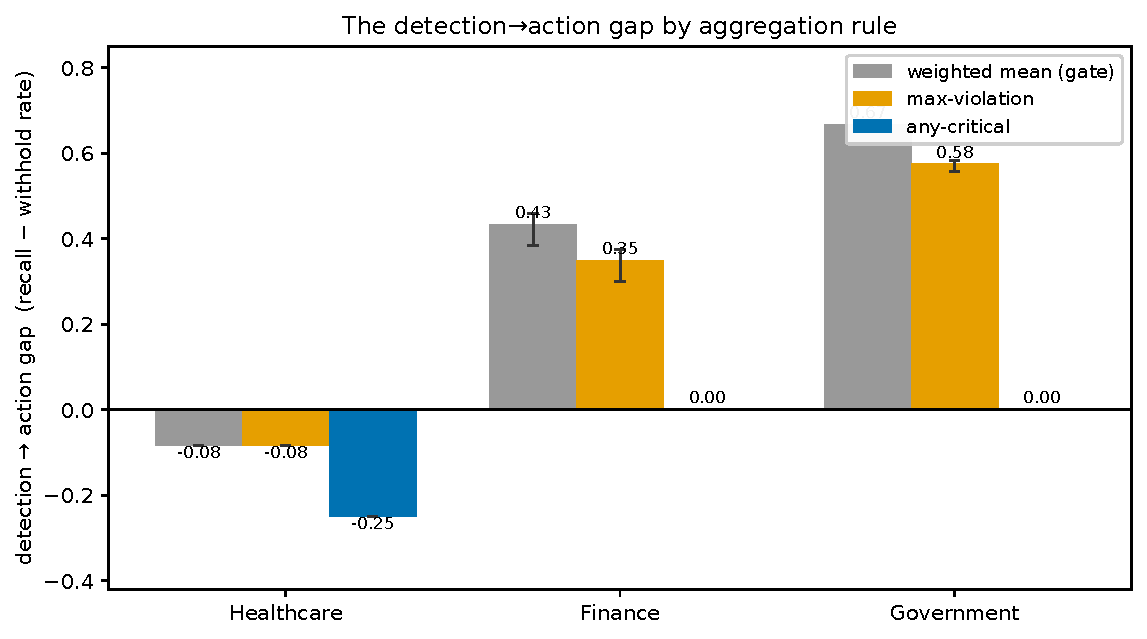
\includegraphics[width=0.49\textwidth]{figA1_gap_by_rule.pdf}
\hfill
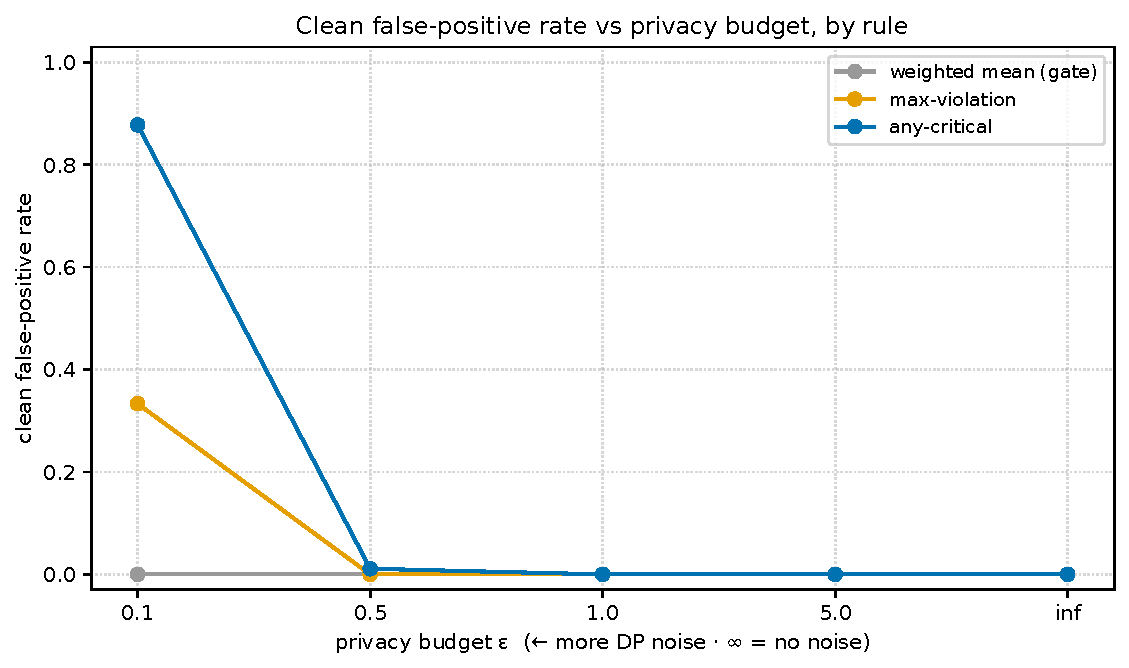
\includegraphics[width=0.49\textwidth]{figA2_fpr_vs_epsilon.pdf}
\caption{\textbf{Aggregation-rule ablation.} Left: the detection$\rightarrow$action
gap closes under \texttt{any-critical}. Right: its clean false-positive rate is
free for $\varepsilon\geq0.5$ but explodes at $\varepsilon{=}0.1$.}
\label{fig:ablation}
\end{figure}

\subsection{Privacy--utility and a DP-robust label detector}

Validating on differentially private summaries trades precision for recall as
$\varepsilon$ falls: clean-data false-flag rate is $0.0$ at every $\varepsilon\geq1$
but rises toward $1.0$ at $\varepsilon{=}0.1$, giving a usable knee at
$\varepsilon\geq0.5$. This is the most technically
original single piece and is reported as an FPR/recall-vs-$\varepsilon$ sweep.

The gate's marginal label-rate detector is \emph{provably} blind to symmetric label
noise on a balanced target: the post-flip positive rate is
$p' = p + r(1-2p)\to p$ as $p\to 0.5$, so finance ($p\approx0.42$) yields recall
$0.00$ at every $\varepsilon$. We add a \emph{confident-learning} detector~\citep{northcutt2021confidentlearning}:
a per-source, cross-validated self-disagreement rate (a bounded proportion in
$[0,1]$ released under Laplace noise; we report its DP accounting as approximate
below), flagged against the cross-source median.
It closes the blind spot (finance symmetric-noise recall $0.00\to0.63$) and,
crucially, is \textbf{DP-robust}: recall holds as $\varepsilon$ falls to $0.1$
(finance $0.63\to0.57$; healthcare and government stay $1.00$), the opposite of the
divergence detector's $\varepsilon{=}0.1$ false-flag blowup
(Fig.~\ref{fig:dp-robust}). The clean self-disagreement standard deviation is tiny
(finance $0.0073$, others ${\sim}0.001$), so the $0.05$ flag threshold separates
clean from noisy with wide margin.

\begin{figure}[t]
\centering
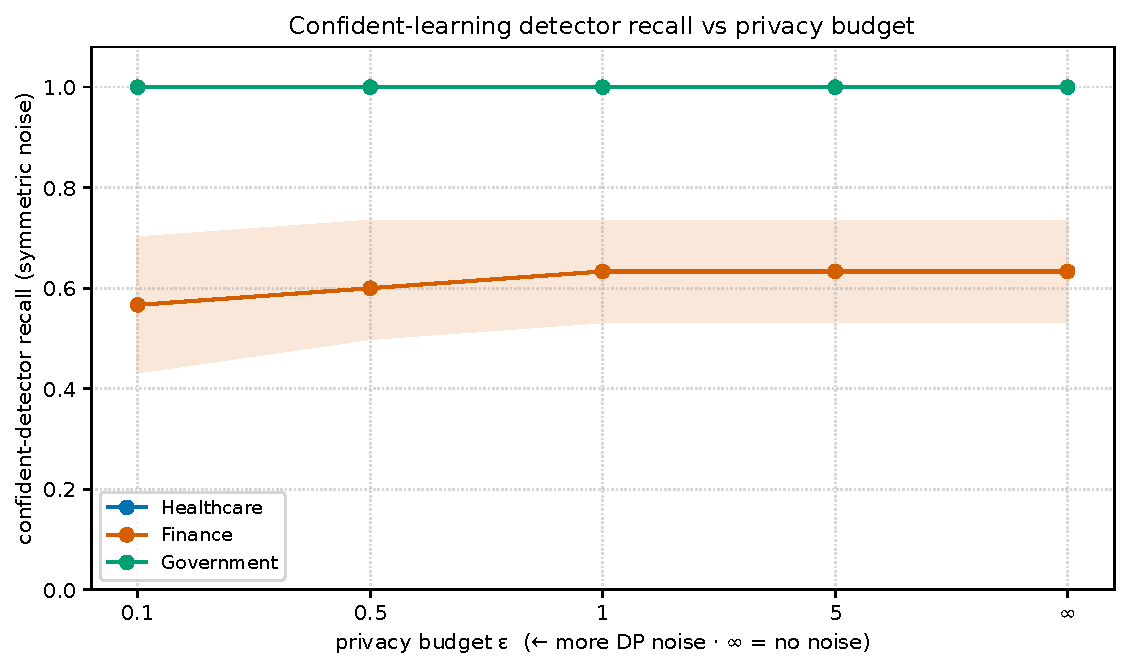
\includegraphics[width=0.72\textwidth]{figE1_confident_epsilon.pdf}
\caption{\textbf{The confident-learning detector is DP-robust.} Recall holds as
$\varepsilon$ falls to $0.1$; bands are seed-level bootstrap 95\% CIs.}
\label{fig:dp-robust}
\end{figure}

\paragraph{DP accounting (approximate).} The self-disagreement statistic is a
proportion in $[0,1]$ released under Laplace noise. A clean bound is not immediate:
because one row participates both in training a cross-validation fold-model and in
being evaluated by it, the statistic's sensitivity is not simply $1/n$ and the
fold-models are not strict post-processing of a differentially private release. We
therefore treat the released scalar as \emph{DP-style} (noised with the Laplace
mechanism) rather than claim a proven $\varepsilon$-DP guarantee, and a rigorous
accounting of the cross-validation coupling is future work. Where we call the
detector ``DP-robust'' (Fig.~\ref{fig:dp-robust}) we mean the empirical observation
that its recall holds as $\varepsilon$ falls, not a formal privacy bound.

\subsection{Downstream: calibration, not accuracy}

An aggregate-AUC downstream arm was uninformative (the corruption barely moved
AUC); redesigned with subgroup and calibration metrics, the finding is that
\textbf{label noise is a calibration failure invisible to AUC}: government
expected calibration error rises $0.046\to0.288$ while AUC holds $0.928\to0.927$ ---
that scales with severity, and the gate recovers the modes it withholds (structural
to the clean-only oracle) but not those it only flags (label)
(Figs.~D1--D3). Gating changes AUC by $|\Delta|<0.005$
everywhere: its value is governance and calibration, not an accuracy lift. We state
this as an honest negative.

\subsection{Baselines: the edge is the layer, not the checks}\label{sec:baselines}

Table~\ref{tab:baselines} compares the gate to Great
Expectations~\citep{greatexpectations} and Deequ~\citep{schelter2018deequ}, both
run on the \emph{same} degraded sources with reference-derived thresholds (TFDV was
omitted for packaging reasons on current Python). On structural and completeness
all three tie at recall $1.0$, and we claim no raw-check novelty. The split is
elsewhere: Deequ (constraints) is the most precise (0.000 clean false-flag) but
flags no label corruption; Great Expectations (expectations) catches more but
false-flags a third of clean healthcare sources; the gate sits at the good corner
(rare-label recall $1.0$ \emph{and} 0.000 clean false-flag). Critically,
\emph{every} baseline misses balanced-label symmetric noise on finance (gate
$0.0$, GE $0.2$, Deequ $0.0$), the blind spot the confident-learning detector
closes. The gate's advantage is the cross-source, differentially private,
decision layer, not any individual check.

\begin{table}[t]
\centering
\caption{Detection recall by mode (severity high, $\varepsilon{=}\infty$),
healthcare / finance / government.}
\label{tab:baselines}
\begin{tabular}{lccc}
\toprule
Mode & Gate & Great Expectations & Deequ \\
\midrule
Structural     & 1.0 / 1.0 / 1.0 & 1.0 / 1.0 / 1.0 & 1.0 / 1.0 / 1.0 \\
Completeness   & 1.0 / 1.0 / 1.0 & 1.0 / 1.0 / 1.0 & 1.0 / 1.0 / 1.0 \\
Distributional & 1.0 / 0.8 / 1.0 & 1.0 / 1.0 / 1.0 & 1.0 / 1.0 / 1.0 \\
Label          & 1.0 / \textbf{0.0} / 1.0 & 1.0 / \textbf{0.2} / 1.0 & \textbf{0.0 / 0.0 / 0.0} \\
\midrule
Clean false-flag & 0.00 / 0.00 / 0.00 & \textbf{0.33} / 0.07 / 0.00 & 0.00 / 0.00 / 0.00 \\
\bottomrule
\end{tabular}
\end{table}

\subsection{Cross-domain transfer and the NIST mapping}

Detection recall is roughly portable across domains, but thresholds are
\emph{not}: calibrating the distributional threshold on one domain and applying it
to another preserves recall (mean $0.69\to0.67$) while inflating the clean
false-flag rate (mean $0.22\to0.44$); healthcare's tight threshold applied to
finance/government drives false-flags to $0.98$/$1.00$
(Fig.~\ref{fig:transfer}). The ``industry-agnostic'' claim must therefore be
stated as \emph{each domain needs its own clean-source calibration}; the retuning
cost is false positives, not lost recall. We map the measured behaviors
(detection, withholding, privacy--utility, transfer) to specific NIST AI RMF
MEASURE subcategories as governance-facing connective tissue
(Table~\ref{tab:measure}), stated at subcategory granularity and defended cell by
cell; it is not claimed as a research contribution.

\begin{figure}[t]
\centering
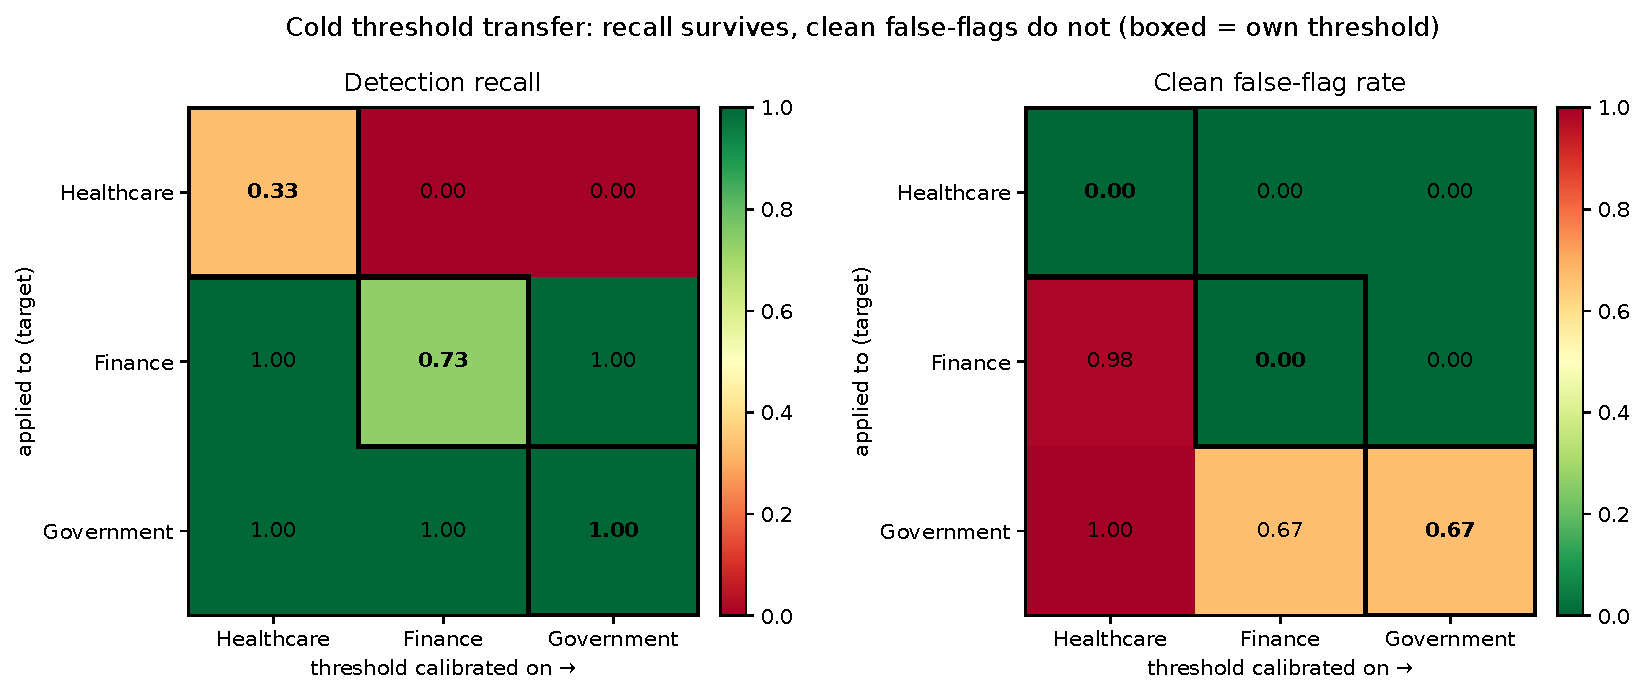
\includegraphics[width=0.82\textwidth]{figT1_threshold_transfer.pdf}
\caption{\textbf{Cold threshold transfer.} Recall survives transfer (left);
clean false-flags do not (right): a mismatched threshold approaches 1.0. Boxed =
own threshold.}
\label{fig:transfer}
\end{figure}

\begin{table}[t]
\centering
\caption{Mapping measured gate behaviors to NIST AI RMF MEASURE subcategories;
IDs and wording verified against NIST AI 100-1~\citep{nistairmf2023} (Table~3,
pp.~29--31). The gate measures the \emph{training data} before a model exists ---
an upstream instantiation of MEASURE's documented-TEVV intent, so each cell is a
``measured and documented'' claim, not risk elimination (MANAGE is out of scope).}
\label{tab:measure}
\small
\begin{tabular}{p{0.45\textwidth}cp{0.33\textwidth}}
\toprule
Measured gate behavior & MEASURE & What it lets one document \\
\midrule
Schema / dtype / range validity checks & 2.1 & Data validity via a versioned, documented test suite \\
Completeness thresholds (null fraction, row count) & 2.5 & Coverage / generalizability limits; missing subpopulations surfaced \\
Cross-source distributional divergence (JS) & 2.11 & Population skew / covariate shift across sources \\
Label-rate check $+$ confident-learning detector & 2.3 & Label integrity as a documented assurance criterion \\
Readiness score $\rightarrow$ \textsc{ready}/\textsc{fixable}/\textsc{exclude} & 1.1 & A single pre-deployment go/no-go metric, documented \\
DP-noised quality reports ($\varepsilon$ budget) & 2.10 & Privacy risk of the measurement process itself \\
Documented blind spots (detection $\neq$ action) & 1.1, 2.13 & Unmeasurable risks documented; TEVV effectiveness evaluated \\
Independent human incident coding (Cohen's $\kappa$) & 1.3 & Non--front-line assessors validate the measurement rule \\
\bottomrule
\end{tabular}
\end{table}

\subsection{Incident-coding reliability: an honest negative}

We double-coded a seeded 30-incident sample (machine vs.\ an independent human
coder). The \emph{coarse} filter is reliable: the human judged 28 of 30 sampled
incidents to be genuine data-readiness failures (filter precision $0.933$). The
\emph{fine} coding is not: assigned-mode agreement is $0.233$ (Cohen's
$\kappa=0.082$) and detectability agreement $0.333$ ($\kappa=0.038$), both near
chance, because the machine coder systematically over-assigns \emph{distributional}
and \emph{partial}. We therefore do \emph{not} claim the fine mode proportions as a
reliable measurement; we use the taxonomy as a qualitative organizing frame and
rely on the human-validated filter precision. AIID reports are media-derived and
root cause is often under-determined, which is consistent with low fine-coding
reliability. ($n{=}30$, no adjudication. A blind intra-rater re-code by the same
coder after a washout agreed with the first pass no better than chance (mode
$\kappa{=}{-}0.05$, detectability $\kappa{=}{-}0.14$), so the \emph{fine} coding is
unstable even within a single coder, not only between the machine and a human. We
therefore rely on the coarse, human-validated filter precision rather than the mode
proportions.)

\section{Limitations and scope}

(1) Gating yields no downstream accuracy lift here; its value is governance and
calibration. (2) The symmetric-label blind spot on balanced targets is provable,
not incidental; the confident-learning detector addresses it but its DP accounting
is approximate. (3) Thresholds do not transfer cold across domains. (4) The
fine-grained incident coding is not reliable (above). (5) Cross-source and
provenance taxonomy modes are not row-injectable and are out of scope for this
harness. We report each of these rather than hide them, consistent with the
detectability-boundary framing.

\section{Conclusion}

Pre-training data-readiness validation helps most when its signals feed a decision
and a governance process. It misleads when a composite score turns ``detected''
into ``allowed'' and no one notices. We measured that gap, showed it is a fixable
but privacy-sensitive design choice, mapped the privacy--utility boundary, added a
DP-robust detector for a provable blind spot, and tied the whole to NIST AI RMF
MEASURE. The work is the integration, and the honest account of where it stops.

\paragraph{Reproducibility.} All figures and numbers regenerate from committed
CSVs with fixed seeds via the \texttt{experiments/analyze*.py} scripts; the gate is
reused unmodified, every detector/metric is an additive extension, and a
verification log records each run. Sources by artifact:
Fig.~\ref{fig:spine} and the downstream figures (Figs.~D1--D3) from
\texttt{crossdomain\_*.csv} and \texttt{downstream\_*.csv};
Fig.~\ref{fig:ablation} from \texttt{aggregation\_*.csv};
Fig.~\ref{fig:dp-robust} from \texttt{label\_epsilon\_*.csv};
Fig.~\ref{fig:transfer} from \texttt{threshold\_transfer\_summary.csv};
Table~\ref{tab:baselines} from \texttt{baselines\_summary.csv} and
\texttt{crossdomain\_*.csv}. The composite readiness rule is
\texttt{src/gate/readiness.py}.

\bibliographystyle{plainnat}
\bibliography{refs}

\end{document}
